\subsection{Tema 1}
\begin{enumerate}
  \item[1.3] \label{1.13} Un  computador  tarda  100  segundos  en  ejecutar  un  programa  de  simulación  de  una  red  de  interconexión  para  multicomputadores.  El  programa  dedica  el 30\% en hacer operaciones de aritmética entera, el 60\% en hacer operaciones de aritmética  en  coma  flotante,  mientras  que  el  resto  se  emplea  en  operaciones  de  entrada/salida.  Calcule  la  ganancia  en  velocidad  y  el  tiempo  de  ejecución  si  las  operaciones  aritméticas  enteras  y  reales  se  mejoran de  manera  simultánea  2  y  3  veces, respectivamente.
	\begin{solution}
		\begin{figure}[H]
			\centering
			\begin{tikzpicture}[arrow/.style = {thick,-stealth}]
				\tikzset{set/.style={draw,rectangle,inner sep=0pt,align=center}}

				\node[fit={(0,0) (1,2.2)}, inner sep=0pt, draw=black, thick, fill=blue!20, text centered] (es) {\footnotesize E/S (\tiny $0.1*t_O=10s$)};
				\node[fit={(1,0) (7,2.2)}, inner sep=0pt, draw=black, thick, fill=green!20, text centered] (float) {Coma flotante (\footnotesize $0.6*t_O=60s$)};
				\node[fit={(7,0) (10,2.2)}, inner sep=0pt, draw=black, thick, fill=blue!20, text centered] (int) {Enteros (\footnotesize $0.3*t_O=30s$)};

				\node[fit={(0,-5) (1,-2)}, inner sep=0pt, draw=black, thick, fill=blue!20, text centered] (esm) {\footnotesize E/S (\tiny $0.1*t_O=10s$)};

				\node[fit={(1,-5) (3,-2)}, inner sep=0pt, draw=black, thick, fill=green!20, text centered] (floatm) {Coma flotante (\footnotesize $\frac{0.6*t_O}{3}=0.2*t_O=20s$)};

				\node[fit={(3,-5) (4.5,-2)}, inner sep=0pt, draw=black, thick, fill=blue!20, text centered] (intm) {Enteros (\footnotesize $\frac{0.3*t_O}{2}=0.15*t_O=30s$)};

				\draw [arrow] (1,0) -- (1,-2);
				\draw [arrow] (7,0) -- node [left] {\tiny $3$ veces más pequeño} (3,-2);
				\draw [arrow] (10,0) -- node [below right] {\tiny $2$ veces más pequeño} (4.5,-2);

				\draw [decorate,decoration={brace,amplitude=10pt, raise=2.5pt}]	(0,2.2) -- (10,2.2) node [black, midway, sloped, above=0.5cm] {Tiempo original $t_O=100s$};

				\draw [decorate,decoration={brace,amplitude=10pt, raise=2.5pt, mirror}]	(0,-5) -- (4.5,-5) node [black, midway, sloped, below=0.5cm] {Tiempo mejorado $t_M=10+20+15=45s$};

			\end{tikzpicture}
		\end{figure}
		Por último, calculamos el \textit{speedup}:
		\[
		S=\frac{v_M}{v_O}=\frac{t_O}{t_M}=\frac{100 s}{45 s}=2.22
		\]
		Por tanto, el tiempo total será de $45s$ y el \textit{speedup} es 2.2 (un 220\% más rápido).

	\end{solution}
	\item[1.13] \label{1.13} Una aplicación informática se ejecuta en un computador durante un total de 70 segundos. Mediante el uso de un monitor de actividad se ha podido saber que  el  85\%  del  tiempo  se  utiliza  la  CPU,  mientras  que  el  resto  del  tiempo  se  hace  uso del disco duro. Determine cuántas veces debe ser, como mínimo, más rápido un procesador que cuesta el doble que el procesador actual para que hubiese valido la pena  comprarlo  en  lugar  de  éste  ateniéndonos  a  la  relación  prestaciones  del sistema/coste de la CPU.
	\begin{solution}
		\begin{figure}[H]
			\centering
			\begin{tikzpicture}[arrow/.style = {thick,-stealth}]
				\tikzset{set/.style={draw,rectangle,inner sep=0pt,align=center}}

				% Original

				\node[fit={(0,0) (1.5,2)}, inner sep=0pt, draw=black, thick, fill=blue!20, text centered] (hdd) {\footnotesize HDD (\tiny $0.15*t_O=10.5s$)};
				\node[fit={(1.5,0) (10,2)}, inner sep=0pt, draw=black, thick, fill=green!20, text centered] (cpu) {CPU ($0.85*t_O=59.5s$)};

				% Mejorado
				\node[fit={(0,-4) (1.5,-2)}, inner sep=0pt, draw=black, thick, fill=blue!20, text centered] (hddm) {\footnotesize HDD (\tiny $0.15*t_O=10.5s$)};

				\node[fit={(1.5,-4) (6,-2)}, inner sep=0pt, draw=black, thick, fill=green!20, text centered] (cpum) {CPU ($\frac{0.85*t_O}{k}=\frac{59.5}{k}s$)};


				\draw [arrow] (1.5,0) -- (1.5,-2);
				\draw [arrow] (10,0) -- node [below right] {\footnotesize $k$ veces más pequeño} (6,-2);

				\draw [decorate,decoration={brace,amplitude=10pt, raise=2.5pt}]	(0,2) -- (10,2) node [black, midway, sloped, above=0.5cm] {Tiempo original $t_O=70s$};

				\draw [decorate,decoration={brace,amplitude=10pt, raise=2.5pt, mirror}]	(0,-4) -- (6,-4) node [black, midway, sloped, below=0.5cm] {Tiempo mejorado $t_M$};

			\end{tikzpicture}
		\end{figure}
		Se debe cumplir que:
		\[
			\frac{Prestaciones(M)}{Coste(CPU_M)} > \frac{Prestaciones(O)}{Coste(CPU_O)}
		\]
		Como $Coste(CPU_M)=2*Coste(CPU_O)$:
		\[
			\frac{Prestaciones(M)}{2*Coste(CPU_O)} > \frac{Prestaciones(O)}{Coste(CPU_O)}	\implies Prestaciones(M) > 2*Prestaciones(O)
		\]
		Es decir, para que salga rentable gastarme el doble en una CPU, las prestaciones deben (como mínimo) duplicarse. Por tanto:
		\[
			v_M>2*v_O \implies \frac{v_M}{v_O} > 2 \implies S > 2 \implies \frac{t_O}{t_M} > 2 \implies \frac{70 s}{10.5 s + \frac{59.5 s}{k}} > 2 \implies k > 2.43
		\]
		Por tanto, el procesador debe ser, como mínimo, 2.43 veces más rápido.
	\end{solution}
	\newpage
	\item[1.11] \label{1.11} Ante la necesidad de reducir el tiempo de ejecución de un programa de cálculo de trayectorias espaciales, un equipo de arquitectos de computadores ha diseñado un nuevo procesador que mejora 15 veces la ejecución de las operaciones de coma flotante. El programa, cuando se ejecuta utilizando este nuevo procesador, emplea el 65 \% del tiempo en la realización de operaciones de coma flotante.
	\begin{enumerate}
		\item Calcule la fracción de tiempo durante el cual se utilizaba la coma flotante en el sistema con el procesador original.
		\item Indique  cuál  es  la  ganancia  en  velocidad global  conseguida  por  el  nuevo  procesador.
	\end{enumerate}
	\begin{solution}
		Tenemos que prestar mucha atención al enunciado, ya que no nos dan el tiempo original como de costumbre, sino el mejorado. Por tanto, debemos seguir el planteamiento inverso al habitual:

		\begin{figure}[H]
			\centering
			\begin{tikzpicture}[arrow/.style = {thick,-stealth}]
				\tikzset{set/.style={draw,rectangle,inner sep=0pt,align=center}}

				% Mejorado

				\node[fit={(0,0) (3.5,2)}, inner sep=0pt, draw=black, thick, fill=blue!20, text centered] (restom) {\footnotesize Resto ($0.35*t_M$)};
				\node[fit={(3.5,0) (6,2)}, inner sep=0pt, draw=black, thick, fill=green!20, text centered] (cpum) {CPU ($0.65*t_M$)};

				% Original
				\node[fit={(0,-4) (3.5,-2)}, inner sep=0pt, draw=black, thick, fill=blue!20, text centered] (hdd) {\footnotesize Resto ($(1-f)*t_O$)};

				\node[fit={(3.5,-4) (10,-2)}, inner sep=0pt, draw=black, thick, fill=green!20, text centered] (cpu) {CPU ($f*t_O$)};


				\draw [arrow] (3.5,0) -- (3.5,-2);
				\draw [arrow] (6,0) -- node [below left] {\footnotesize 15 veces mayor} (10,-2);

				\draw [decorate,decoration={brace,amplitude=10pt, raise=2.5pt}]	(0,2) -- (6,2) node [black, midway, sloped, above=0.5cm] {Tiempo mejorado $t_M$};

				\draw [decorate,decoration={brace,amplitude=10pt, raise=2.5pt, mirror}]	(0,-4) -- (10,-4) node [black, midway, sloped, below=0.5cm] {Tiempo original $t_O$};
			\end{tikzpicture}
		\end{figure}
		Nos piden calcular $f$ y $S$. Si comenzamos por $S$, podremos calcular $f$ de forma sencilla:
		\[
			S=\frac{v_M}{v_O}=\frac{t_O}{t_M}=\frac{0.35*t_M + 0.65*t_M*15}{t_M}=10.1
		\]
		Ahora calculamos $f$:
		\[
			f*t_O=0.65*t_M*15 \implies f*\frac{t_O}{t_M}=0.65*15 \implies f*S=0.65*15 \implies f=0.965
		\]
		Por tanto, $f=0.965$ y $S=10.1$
	\end{solution}
	\newpage
	\item[1.10] \label{1.10} Un equipo de biólogos que investiga sobre clonación de células utiliza el  multiprocesador  ALLIANT  para  ejecutar  un  simulador  que  se  puede  paralelizar  en  una  fracción  f  de  su  tiempo  de  ejecución.  La  figura  adjunta  presenta  la  ganancia  en  velocidad conseguida  por  la  máquina  paralela  en  la  ejecución  del  simulador  para  diferentes valores del número de procesadores (p).
	\begin{figure}[H]
		\centering
		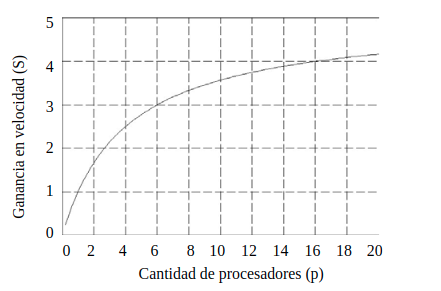
\includegraphics[width=0.5\textwidth]{ej110.png}
	\end{figure}

	\begin{solution}
		\begin{figure}[H]
			\centering
			\begin{tikzpicture}[arrow/.style = {thick,-stealth}]
				\tikzset{set/.style={draw,rectangle,inner sep=0pt,align=center}}

				% Original

				\node[fit={(0,0) (3.5,2)}, inner sep=0pt, draw=black, thick, fill=blue!20, text centered] (nopar) {No paralelizable ($(1-f)*t_O$)};
				\node[fit={(3.5,0) (10,2)}, inner sep=0pt, draw=black, thick, fill=green!20, text centered] (par) {Paralelizable ($f*t_O$)};

				% Mejorado
				\node[fit={(0,-4) (3.5,-2)}, inner sep=0pt, draw=black, thick, fill=blue!20, text centered] (noparm) {No paralelizable ($(1-f)*t_O$)};

				\node[fit={(3.5,-4) (7,-2)}, inner sep=0pt, draw=black, thick, fill=green!20, text centered] (cpum) {Paralelizable ($f*\frac{t_O}{p}$)};


				\draw [arrow] (1.5,0) -- (1.5,-2);
				\draw [arrow] (10,0) -- node [below right] {\footnotesize $p$ veces más pequeño} (6,-2);

				\draw [decorate,decoration={brace,amplitude=10pt, raise=2.5pt}]	(0,2) -- (10,2) node [black, midway, sloped, above=0.5cm] {Tiempo original $t_O$};

				\draw [decorate,decoration={brace,amplitude=10pt, raise=2.5pt, mirror}]	(0,-4) -- (7,-4) node [black, midway, sloped, below=0.5cm] {Tiempo mejorado $t_M$};

				\draw [decorate,decoration={brace,amplitude=10pt, raise=2.5pt, mirror}]	(10.2,0) -- (10.2,2) node [black,midway,xshift=2cm] {1 procesador};

				\draw [decorate,decoration={brace,amplitude=10pt, raise=2.5pt, mirror}]	(10.2,-4) -- (10.2,-2) node [black,midway,xshift=2cm] {$p$ procesadores};

			\end{tikzpicture}
		\end{figure}
		\begin{enumerate}
			\item[a)] ¿Cuál es la fracción paralelizable f  del programa de simulación?
			\vspace{0.5cm}
				Tomamos un punto cualquiera de la gráfica y aplicamos la Ley de Amdahl para obtener $f$. Por ejemplo, $p=6 \implies S=3$
			\[
				S=\frac{1}{1-f+\frac{f}{p}} \implies 3=\frac{1}{1-f+\frac{f}{6}} \implies f=0.8
			\]
			Por tanto, $f=0.8$.
		\item[b)] Si  la  parte  secuencial (=no  paralelizable)  del  simulador  se  ejecuta  en  65 segundos,  ¿cuánto  tiempo  han  de  esperar  los  biólogos  para  obtener  los  resultados de la simulación con una configuración de 6 procesadores?
		\vspace{0.5cm}
			\begin{figure}[H]
				\centering
				\begin{tikzpicture}[arrow/.style = {thick,-stealth}]
					\tikzset{set/.style={draw,rectangle,inner sep=0pt,align=center}}

					% Original

					\node[fit={(0,0) (3.5,2)}, inner sep=0pt, draw=black, thick, fill=blue!20, text centered] (nopar) {No paralelizable ($(1-f)*t_O=65 s$)};
					\node[fit={(3.5,0) (10,2)}, inner sep=0pt, draw=black, thick, fill=green!20, text centered] (par) {Paralelizable ($f*t_O$)};

				\end{tikzpicture}
			\end{figure}
			Como sabemos que $(1-f)*t_O=65 s$ y tenemos $f$, calculamos $t_O$:
			\[
			(1-0.8)*t_O=65 s \implies t_O=\frac{65}{0.2}s=325 s
			\]
			Ahora, para calcular $t_M$, obtenemos la ganancia con $p=6$ ($S=3$). Por último, aplicamos la fórmula de la ganancia:
			\[
				S=\frac{t_O}{t_M} \implies 3 = \frac{325 s}{t_M} \implies t_M = \frac{325}{3}s=108.33s
			\]
			Por tanto, habrá que esperar 108.33 s.
		\item[c)] Los  científicos  pretenden  obtener  resultados  del  simulador  en  un  tiempo  máximo de veinte segundos sin modificar el código del programa. Si el sistema ALLIANT está preparado para ampliar el número de procesadores hasta p = 30, ¿podrán conseguir los biólogos su objetivo?
		\vspace{0.5cm}

		Comencemos hallando la ganancia mediante la Ley de Amdahl:
		\[
			S=\frac{1}{1-f+\frac{f}{p}}=\frac{1}{1-0.8+\frac{0.8}{30}}=4.41
		\]
		Ahora, aplicamos la fórmula de la ganancia y el valor de $t_O$ obtenido en el apartado a) para obtener $t_M$:
		\[
			S=\frac{t_O}{t_M} \implies t_M=\frac{t_O}{S}\implies t_M=\frac{325s}{4.41}=73.69
		\]
		Como $73.69>20$, podemos afirmar que no será posible lograr el objetivo.
		\item[d)] Un  informático  afirma  que  el  sistema  ALLIANT  podría  conseguir  el  objetivo  anterior con p = 6 procesadores si se reduce a la mitad la fracción secuencial(=no paralelizable) del simulador. ¿Es válida esta propuesta?\\
		\vspace{0.5cm}
			Si reducimos a la mitad el tiempo no paralelizable, tendríamos el siguiente escenario:
			\begin{figure}[H]
				\centering
				\begin{tikzpicture}[arrow/.style = {thick,-stealth}]
					\tikzset{set/.style={draw,rectangle,inner sep=0pt,align=center}}

					% Original

					\node[fit={(0,0) (3.5,2)}, inner sep=0pt, draw=black, thick, fill=blue!20, text centered] (nopar) {No paralelizable ($(1-f)*t_O=65s$)};
					\node[fit={(3.5,0) (10,2)}, inner sep=0pt, draw=black, thick, fill=green!20, text centered] (par) {Paralelizable ($f*t_O$)};

					% Mejorado
					\node[fit={(0,-4) (1.75,-2)}, inner sep=0pt, draw=black, thick, fill=blue!20, text centered] (noparm) {\scriptsize No paralelizable ($\frac{(1-f)*t_O}{2}=32.5$)};

					\node[fit={(1.75,-4) (7,-2)}, inner sep=0pt, draw=black, thick, fill=green!20, text centered] (cpum) {Paralelizable ($f*\frac{t_O}{6}$)};


					\draw [arrow] (3.5,0) -- node [below right] {\footnotesize La mitad} (1.75,-2);
					\draw [arrow] (10,0) -- node [below right] {\footnotesize $6$ veces más pequeño} (7,-2);

					\draw [decorate,decoration={brace,amplitude=10pt, raise=2.5pt}]	(0,2) -- (10,2) node [black, midway, sloped, above=0.5cm] {Tiempo original $t_O$};

					\draw [decorate,decoration={brace,amplitude=10pt, raise=2.5pt, mirror}]	(0,-4) -- (7,-4) node [black, midway, sloped, below=0.5cm] {Tiempo mejorado $t_M$};

					\draw [decorate,decoration={brace,amplitude=10pt, raise=2.5pt, mirror}]	(10.2,0) -- (10.2,2) node [black,midway,xshift=2cm] {1 procesador};

					\draw [decorate,decoration={brace,amplitude=10pt, raise=2.5pt, mirror}]	(10.2,-4) -- (10.2,-2) node [black,midway,xshift=2cm] {$6$ procesadores};

				\end{tikzpicture}
			\end{figure}
			Realmente no tenemos que realizar cálculos. Vemos que la parte no paralelizable es de $32.5s$ y como $32.5>20$, la propuesta no es válida.
		\end{enumerate}
	\end{solution}
\end{enumerate}
